% Déclaration du type de document (report, book, paper, etc...)
\documentclass[a4paper]{paper} 
 
% Package pour avoir Latex en français
\usepackage[utf8]{inputenc}
\usepackage[T1]{fontenc}
 
% Quelques packages utiles
\usepackage{listings} % Pour afficher des listings de programmes
\usepackage{graphicx} % Pour afficher des figures
\usepackage{amsthm}   % Pour créer des théorèmes et des définitions
\usepackage{amsmath}
\usepackage{microtype} % Optical margins FTW
\usepackage{url}
\usepackage{booktabs} % Allows the use of \toprule, \midrule and \bottomrule in tables for horizontal lines
\usepackage{siunitx}
\usepackage{floatrow}
\usepackage{caption}
\usepackage{subcaption}
\usepackage{mhchem}
\usepackage[acronym,smallcaps]{glossaries}


% Début du document
\begin{document}
\begin{titlepage}

\newcommand{\HRule}{\rule{\linewidth}{0.5mm}} % Defines a new command for the horizontal lines, change thickness here

\center % Center everything on the page 
%----------------------------------------------------------------------------------------
%	HEADING 
%----------------------------------------------------------------------------------------
\textsc{\LARGE Club Vaudois de Robotique Autonome}\\[1.5cm] 

%----------------------------------------------------------------------------------------
%	TITLE 
%----------------------------------------------------------------------------------------
\HRule \\[0.4cm]
{ \huge \bfseries Eurobot 2014 : Pilot Study}\\[0.4cm] % Title of your document
\HRule \\[1.5cm]
 
%----------------------------------------------------------------------------------------
% LOGO EPFL
%----------------------------------------------------------------------------------------
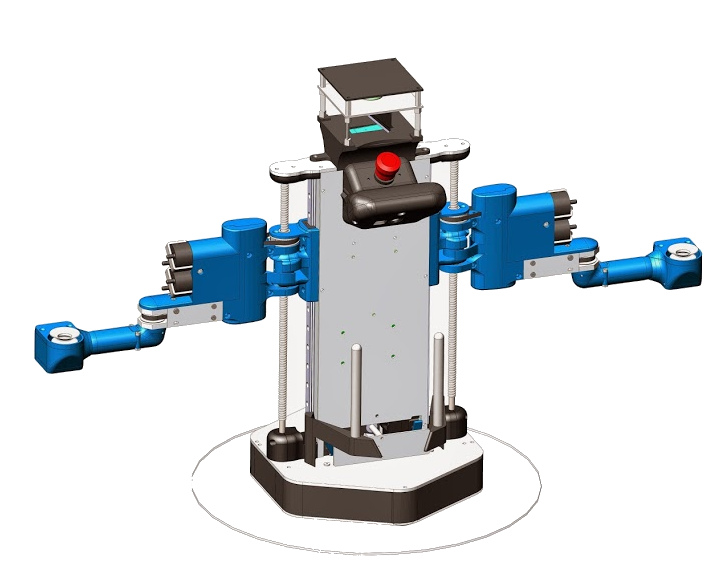
\includegraphics[width=\textwidth]{images/Debra_IV_1}\\[2cm] 

%----------------------------------------------------------------------------------------
%	AUTHORS 
%----------------------------------------------------------------------------------------

\vfill % Fill the rest of the page with whitespace

{\large \today}
\end{titlepage}



\tableofcontents

\section{General information}
\begin{itemize}
    \item This project study can be published before the contest.
    \item Team name : CVRA (Club Vaudois de Robotique Autonome).
    \item Team location : Renens, Switzerland.
    \item Budget : About 3000 \textsc{chf}, plus sponsors.
\end{itemize}

\section{Robots}
This year the club will engage two robots which are evolutions of previous years' designs.
The first one will have two arms, a differential drive and has code name ``Debra 4''.
The second one will have an holonomic base, and is nicknamed ``Nastya 2''.

\subsection{Debra 4}

\paragraph{Motors}
Debra 4 uses two Faulhaber 2232-012-SR motors, rated at \SI{8.7}{\watt} at \SI{12}{\volt}, overvolted at \SI{14.8}{\volt}.
Those motors allows us to use our max acceleration (wheel slippage) to \SI{0.8}{\meter\per\second}.
All the motors in the robots are driven using custom power electronics.

\paragraph{Positioning}
Debra 4 will use a standard, encoder-based odometry to find its position on the table.
We will also use an inertial measurement unit to have an additional source of information.
These two techniques will be merged using a Kalman filter.

\paragraph{Opponent detection}
We have planned to build an optical absolute positioning beacon system, but it may not be ready for the contest due to the complexity of the project.
If we cannot make it in time, we will fall back on last year's beacon system (fig. \ref{fig:balise}).
The relative simplicity of this second design makes it very reliable and easy to implement, which guarantees that it will be ready for the Belgium and Switzerland contests.

\begin{figure}[h]
    \begin{center}
        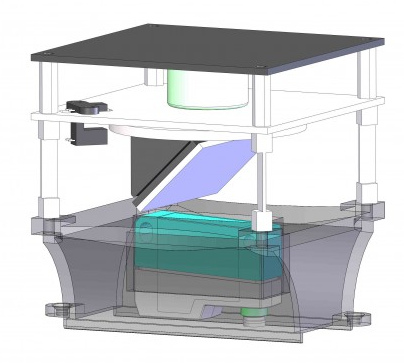
\includegraphics[width=0.6\textwidth]{images/Balise}
        \caption{Fallback beacon system.
            A reflex-type industrial sensor is mounted in the base (blue).
            It emits a LED beam (not laser), which is reflected on the rotating mirror (purple).
            A reflector is placed on the opponent robot, which allows for reliable detection.
            An index sensor (upper left, black) allows the robot to know the relative angle to opponent.
        }
        \label{fig:balise}
    \end{center}
\end{figure}


\section{Team members}
\begin{itemize}
    \item Antoine Albertelli, 21:  Lead developper, Debra 4.
    \item Florian Reinhard, XX:  Lead developper, Nastya 2.
    \item Patrick Spieler, XX:  Inter-board communication.
    \item Pius von Däniken, XX:  Motion planning.
    \item Romain Bersier, 29:  Mechanical engineer, Debra 4.
    \item Boris Pillionnel, 23:  Mechanical engineer, Nastya 2.
    \item Patrick Eugster, 29:  Electrical engineer.
    \item Thierry Prêtre, 21:  Sponsoring.
    \item Mathieu Rouvinez, XX:  Machining and mathematical wizardry.
    \item Guillaume:  Il fait quoi ?
    \item Jess:  De même
\end{itemize}




\end{document}
